\section{Cách giải 1: Cân bằng lực}
\begin{enumerate}[label=(\alph*)]
\item Do ròng rọc rất nhẹ và dây thép rất nhẵn nên lực tác dụng lên ròng rọc theo phương song song với cạnh bằng $0$, nói cách khác là dây có phương vuông góc với cạnh.

Khi hệ ở trạng thái cân bằng, ta dễ dàng thấy được lực căng do mỗi dây tác dụng lên $M$ là bằng nhau và có độ lớn là $T=mg$.

Áp dụng định lý con nhím cho đa giác $N$ cạnh, do $l_1=l_2=...=l_N=l$ nên phương trình đã cho trở thành:
\begin{equation}
\vec{\hat{n}_1}+\vec{\hat{n}_2}+...+\vec{\hat{n}_N}=\vec{0}.
\end{equation}

Nhân cả hai vế với $T$ và do $\vec{T_i}$ (vector lực căng dây tương ứng với ròng rọc ở cạnh thứ $i$) song song và cùng chiều với $\vec{\hat{n_i}}$ nên:
\begin{equation}
\vec{T_1} + \vec{T_2}+...+\vec{T_N}=\vec{0}.
\end{equation}
Hay là tổng hợp lực tác dụng lên $M$ bằng $0$ vậy nên vật $M$ ở trạng thái cân bằng tại mọi vị trí bên trong khu vực mà mỗi cạnh chỉ chứa một ròng rọc.

Ta có các vị trí cân bằng ứng với $N=5$ và $N=6$ (các vùng được tô xanh và hồng tương ứng) như hình vẽ sau:
\begin{figure}[H]
\scalebox{0.75}{
\definecolor{fuqqzz}{rgb}{0.9568627450980393,0,0.6}
\definecolor{qqqqff}{rgb}{0,0,1}
\definecolor{ttzzqq}{rgb}{0.2,0.6,0}
\definecolor{zzttqq}{rgb}{0.6,0.2,0}
\begin{tikzpicture}[line cap=round,line join=round,>=triangle 45,x=1cm,y=1cm]
\clip(-8.873415233529899,-3.7005639828456323) rectangle (14.615466183323264,9.59429794121481);
\fill[line width=2pt,color=zzttqq,fill=zzttqq,fill opacity=0.10000000149011612] (-5,0) -- (-2,0) -- (-1.0729490168751576,2.85316954888546) -- (-3.5,4.616525305762879) -- (-5.9270509831248415,2.853169548885461) -- cycle;
\fill[line width=2pt,color=ttzzqq,fill=ttzzqq,fill opacity=0.1] (2,0) -- (5,0) -- (6.5,2.598076211353316) -- (5,5.196152422706633) -- (2,5.196152422706634) -- (0.5,2.5980762113533187) -- cycle;
\fill[line width=2pt,color=qqqqff,fill=qqqqff,fill opacity=0.2] (-4.427050983124842,3.34054909323482) -- (-3.5,3.6417662170641605) -- (-2.5729490168751594,3.3405490932348205) -- (-2,2.551952425056118) -- (-2,1.5771933363574) -- (-2.572949016875158,0.7885966681786997) -- (-3.5,0.4873795443493592) -- (-4.427050983124842,0.7885966681787006) -- (-5,1.5771933363574013) -- (-5,2.55195242505612) -- cycle;
\fill[line width=2pt,color=fuqqzz,fill=fuqqzz,fill opacity=0.45] (3.5,4.330127018922194) -- (5,3.4641016151377544) -- (5,1.7320508075688759) -- (3.5,0.8660254037844383) -- (2,1.7320508075688772) -- (2,3.464101615137757) -- cycle;
\draw [line width=2pt,color=zzttqq] (-5,0)-- (-2,0);
\draw [line width=2pt,color=zzttqq] (-2,0)-- (-1.0729490168751576,2.85316954888546);
\draw [line width=2pt,color=zzttqq] (-1.0729490168751576,2.85316954888546)-- (-3.5,4.616525305762879);
\draw [line width=2pt,color=zzttqq] (-3.5,4.616525305762879)-- (-5.9270509831248415,2.853169548885461);
\draw [line width=2pt,color=zzttqq] (-5.9270509831248415,2.853169548885461)-- (-5,0);
\draw [line width=2pt,color=ttzzqq] (2,0)-- (5,0);
\draw [line width=2pt,color=ttzzqq] (5,0)-- (6.5,2.598076211353316);
\draw [line width=2pt,color=ttzzqq] (6.5,2.598076211353316)-- (5,5.196152422706633);
\draw [line width=2pt,color=ttzzqq] (5,5.196152422706633)-- (2,5.196152422706634);
\draw [line width=2pt,color=ttzzqq] (2,5.196152422706634)-- (0.5,2.5980762113533187);
\draw [line width=2pt,color=ttzzqq] (0.5,2.5980762113533187)-- (2,0);
\draw (3,-0.3) node[anchor=north west] {$N=6$};
\draw (-4,-0.3) node[anchor=north west] {$N=5$};
\end{tikzpicture}
}
\centering
\caption{}
\label{figs:S1_01}
\end{figure}
Ta vẽ các vị trí trên bằng cách từ một đỉnh ta hạ đường thẳng vuông góc với hai cạnh kề với đỉnh đó (do dây luôn vuông góc với cạnh và ta xác định vùng mà ròng rọc nằm trên cạnh đó bằng cách kẻ đường vuông góc với cạnh từ hai đầu mút của mỗi cạnh, khi đó không gian nằm giữa hai đường thẳng vừa kẻ là vùng mà ròng rọc vẫn nằm trên cạnh đó) ta dễ dàng tìm được khu vực mà vật $M$ sẽ cân bằng (Ngoài ra, ta có thể để ý rằng đối với $N$ lẻ thì khu vực đó có dạng $2N$ giác đều còn $N$ chẵn thì khu vực đó có dạng $N$ giác đều)
\item Ta cũng lập luận tương tự ý trên ta suy ra được rằng lò xo vuông góc với cạnh. Ta kí hiệu $d_1,d_2,d_3$ lần lượt là khoảng cách từ $M$ đến các cạnh có chiều dài $l_1,l_2,l_3$.

Sử dụng định lí con nhím cho tam giác:
\begin{equation}
l_1\vec{\hat{n}_1}+l_2\vec{\hat{n}_2}+l_3\vec{\hat{n}_3}=\vec{0}.
\end{equation}

Lực đàn hồi ứng với cạnh thứ $i$ hướng song song và cùng chiều với vector $\vec{\hat{n}_i}$. Theo định luật Hooke, ta có lực đàn hồi: $\vec{F_i}=k_id_i\vec{\hat{n}_i}$.

Từ các biếu thức trên, ta được:
\begin{equation}
\label{eq:S1_01}
\dfrac{l_1}{k_1d_1}k_1d_1\vec{\hat{n_1}}+\dfrac{l_2}{k_2d_2}k_2d_2\vec{\hat{n_2}}+\dfrac{l_3}{k_3d_3}k_3d_3\vec{\hat{n_3}}=\vec{0}.
\end{equation}

\begin{equation}
\Longrightarrow\dfrac{l_1}{k_1d_1}\vec{F_1}+\dfrac{l_2}{k_2d_2}\vec{F_2}+\dfrac{l_3}{k_3d_3}\vec{F_3}=\vec{0}.
\end{equation}

Để cân bằng lực, $\vec{F_1}+\vec{F_2}+\vec{F_3}=\vec{0}$:

\begin{equation}
\label{eq:S1_02}
\Longrightarrow \dfrac{l_1}{k_1d_1}=\dfrac{l_2}{k_2d_2}=\dfrac{l_3}{k_3d_3}.
\end{equation}
    \begin{enumerate}[label=(\roman*)]
    \item Trong trường hợp $l_1:l_2:l_3=k_1:k_2:k_3$, ta dễ dàng suy ra được $d_1=d_2=d_3$. Nói cách khác, điểm $M$ khi đó nằm cân bằng ở tâm đường tròn nội tiếp của tam giác.
    \item Trong trường hợp $k_1=k_2=k_3=k$, ta được: 
    \begin{equation}
    \label{eq:S1_03}
    \dfrac{l_1}{d_1}=\dfrac{l_2}{d_2}=\dfrac{l_3}{d_3}.
    \end{equation}
    Khi đó ta thấy được rằng điểm $M$ nằm cân bằng ở điểm Lemoine của tam giác như sau:

    Ta đặt các đỉnh của tam giác là $A,B,C$. Hình chiếu của $M$ lên $BC,CA,AB$ là $M_1,M_2,M_3$. Ta dựng phân giác góc $A$ và lấy điểm $M'$ đối xứng với $M$ qua đường phân giác. Gọi giao điểm của $AM'$ với $BC$ là $A'$ (xem hình vẽ bên dưới).

\begin{figure}[H]    
\centering
% Gradient Info
  
\tikzset {_90k2znmbz/.code = {\pgfsetadditionalshadetransform{ \pgftransformshift{\pgfpoint{89.1 bp } { -128.7 bp }  }  \pgftransformscale{1.32 }  }}}
\pgfdeclareradialshading{_t67nn9g7p}{\pgfpoint{-72bp}{104bp}}{rgb(0bp)=(0.89,0.75,0.75);
rgb(0bp)=(0.89,0.75,0.75);
rgb(12.589285714285714bp)=(0.82,0.01,0.11);
rgb(400bp)=(0.82,0.01,0.11)}
\tikzset{every picture/.style={line width=0.75pt}} %set default line width to 0.75pt        

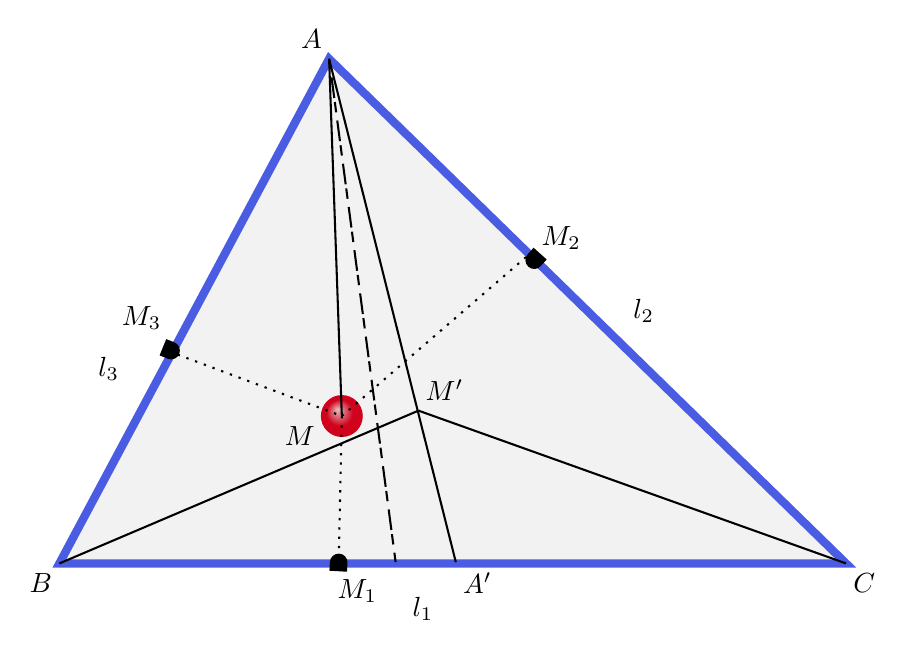
\begin{tikzpicture}[x=0.75pt,y=0.75pt,yscale=-1,xscale=1]
%uncomment if require: \path (0,462); %set diagram left start at 0, and has height of 462

%Shape: Triangle [id:dp3326541587702424] 
\draw  [color={rgb, 255:red, 74; green, 93; blue, 226 }  ,draw opacity=1 ][fill={rgb, 255:red, 128; green, 128; blue, 128 }  ,fill opacity=0.1 ][line width=3]  (179.94,26) -- (429,269.11) -- (50,269.11) -- cycle ;
%Flowchart: Delay [id:dp8143670880210933] 
\draw  [fill={rgb, 255:red, 0; green, 0; blue, 0 }  ,fill opacity=1 ] (101.75,161.68) -- (105.21,163.09) .. controls (107.13,163.87) and (108.05,166.05) .. (107.27,167.97) .. controls (106.49,169.88) and (104.31,170.8) .. (102.39,170.02) -- (98.93,168.61) -- cycle ;
%Flowchart: Delay [id:dp9198941962672681] 
\draw  [fill={rgb, 255:red, 0; green, 0; blue, 0 }  ,fill opacity=1 ] (180.61,272.15) -- (180.83,268.42) .. controls (180.95,266.36) and (182.72,264.78) .. (184.78,264.9) .. controls (186.84,265.02) and (188.42,266.79) .. (188.3,268.86) -- (188.08,272.59) -- cycle ;
%Flowchart: Delay [id:dp3222573149762976] 
\draw  [fill={rgb, 255:red, 0; green, 0; blue, 0 }  ,fill opacity=1 ] (284.07,122.71) -- (281.57,125.5) .. controls (280.19,127.03) and (277.82,127.16) .. (276.29,125.78) .. controls (274.75,124.4) and (274.62,122.04) .. (276,120.5) -- (278.5,117.72) -- cycle ;
%Flowchart: Connector [id:dp4674995309000146] 
\path  [shading=_t67nn9g7p,_90k2znmbz] (176.49,198.1) .. controls (176.49,192.8) and (180.78,188.5) .. (186.08,188.5) .. controls (191.38,188.5) and (195.67,192.8) .. (195.67,198.1) .. controls (195.67,203.39) and (191.38,207.69) .. (186.08,207.69) .. controls (180.78,207.69) and (176.49,203.39) .. (176.49,198.1) -- cycle ; % for fading 
 \draw  [color={rgb, 255:red, 208; green, 2; blue, 27 }  ,draw opacity=1 ][line width=0.75]  (176.49,198.1) .. controls (176.49,192.8) and (180.78,188.5) .. (186.08,188.5) .. controls (191.38,188.5) and (195.67,192.8) .. (195.67,198.1) .. controls (195.67,203.39) and (191.38,207.69) .. (186.08,207.69) .. controls (180.78,207.69) and (176.49,203.39) .. (176.49,198.1) -- cycle ; % for border 

%Straight Lines [id:da2866658385087255] 
\draw    (179.94,26) -- (241,268.5) ;
%Straight Lines [id:da04794658376262384] 
\draw  [dash pattern={on 0.84pt off 2.51pt}]  (107,168.5) -- (186.08,198.1) ;
%Straight Lines [id:da19647849123319838] 
\draw  [dash pattern={on 0.84pt off 2.51pt}]  (186.08,198.1) -- (184.56,268.64) ;
%Straight Lines [id:da7185203893957963] 
\draw  [dash pattern={on 0.84pt off 2.51pt}]  (186.08,198.1) -- (276,120.5) ;
%Straight Lines [id:da4577311492825563] 
\draw  [dash pattern={on 3.75pt off 3pt on 7.5pt off 1.5pt}]  (179.94,26) -- (212,268.5) ;
%Straight Lines [id:da048770005146599904] 
\draw    (179.94,26) -- (186.08,198.1) ;
%Straight Lines [id:da004397076478948825] 
\draw    (50,269.11) -- (223,195.5) ;
%Straight Lines [id:da0889957519920831] 
\draw    (223,195.5) -- (429,269.11) ;

% Text Node
\draw (218.7,283.69) node [anchor=north west][inner sep=0.75pt]    {$l_{1}$};
% Text Node
\draw (325.07,140.28) node [anchor=north west][inner sep=0.75pt]    {$l_{2}$};
% Text Node
\draw (67.23,168.46) node [anchor=north west][inner sep=0.75pt]    {$l_{3}$};
% Text Node
\draw (174.49,201.5) node [anchor=north east] [inner sep=0.75pt]    {$M$};
% Text Node
\draw (177.94,22.6) node [anchor=south east] [inner sep=0.75pt]    {$A$};
% Text Node
\draw (48,272.51) node [anchor=north east] [inner sep=0.75pt]    {$B$};
% Text Node
\draw (431,272.51) node [anchor=north west][inner sep=0.75pt]    {$C$};
% Text Node
\draw (182.61,275.55) node [anchor=north west][inner sep=0.75pt]    {$M_{1}$};
% Text Node
\draw (280.78,119.6) node [anchor=south west] [inner sep=0.75pt]    {$M_{2}$};
% Text Node
\draw (100.55,158.02) node [anchor=south east] [inner sep=0.75pt]    {$M_{3}$};
% Text Node
\draw (243,271.9) node [anchor=north west][inner sep=0.75pt]    {$A'$};
% Text Node
\draw (225,192.1) node [anchor=south west] [inner sep=0.75pt]    {$M'$};


\end{tikzpicture}
\caption{}
\label{figs:S1_02}
\end{figure}

    Do đối xứng qua phân giác góc $A$ nên $M'$ khoảng cách đến $AB$ là $d_2$, cách $AC$ là $d_3$. Từ điều kiện ở trên ta được $d_3l_2=d_2l_3$, hay diện tích các tam giác sau bằng nhau: 
    \begin{equation}
    A_{AM'B}=A_{AM'C}
    \end{equation}
    \begin{equation}
    \Longrightarrow 
    \dfrac{1}{2}l_3AM'\sin{\widehat{BAA'}}=\dfrac{1}{2}l_2AM'\sin{\widehat{CAA'}}.
    \end{equation}
    \begin{equation}
    \Longrightarrow l_3AA'\sin{\widehat{BAA'}}=l_2AA'\sin{\widehat{CAA'}}.
    \end{equation}
    \begin{equation}
    \Longrightarrow A_{AA'B}=A_{AA'C}.
    \end{equation}
    \begin{equation}
    \Longrightarrow A'B=A'C=\dfrac{l_1}{2}.
    \end{equation}
    Điều đó chứng tỏ rằng $A'$ là trung điểm $BC$, nói cách khác $AA'$ là đường trung tuyến ứng với $A$ của tam giác $ABC$ và $AM$ là đường đối trung tương ứng với đỉnh $A$. Tương tự, ta sẽ suy ra được rằng điểm $M$ là giao điểm của ba đường đối trung hay chính là điểm Lemoine.

    
    \end{enumerate}
\end{enumerate}

\textbf{Phổ điểm}
    \begin{center}
    \begin{tabular}{|c|p{8cm}|c|}
    \hline
    \multicolumn{1}{|l|}{Phần} & Nội dung & Điểm thành phần \\ 
    \hline
\multirow{4}{*}{(a)} & Chỉ ra rằng dây vuông góc với các cạnh.
                     & 0.25
                     \\
                     \cline{2-3}
                     & Chỉ ra tất cả các vị trí cân bằng.      
                     & 0.5           
                     \\ 
                     \cline{2-3}
                     & Vẽ hình trường hợp $N = 5$, $N = 6$.        
                     & 0.25           
                     \\
                     \cline{2-3}
                     \hline  
\multirow{4}{*}{(b)} & Chỉ ra rằng lò xo vuông góc với cạnh tam giác.                                       & 0.25             
                     \\
                     \cline{2-3}
                     & Lập luận được biểu thức \eqref{eq:S1_01}. 
                     & 0.25
                     \\
                     \cline{2-3}
                     & Ra được biểu thức \eqref{eq:S1_02}. 
                     & 1.0
                     \\
                     \hline
\multirow{1}{*}{(b)(i)}& Chỉ ra rằng M cân bằng ở tâm đường tròn nội tiếp của tam giác.
                     & 0.5    
                     \\
                     \hline
\multirow{3}{*}{(b)(ii)}
                     &Ra được biểu thức \eqref{eq:S1_03}.     
                     & 0.5
                     \\
                     \cline{2-3}
                     & Chứng minh được M cân bằng ở điểm Lemoine.  
                     & 0.5
                     \\ \hline
                         


    \end{tabular}
    \end{center}

\section{Cách giải 2: Cực tiểu thế năng}
\begin{enumerate}[label=(\alph*)]
\item Ta cũng lập luận như cách 1 để suy ra rằng dây vuông góc với các cạnh. Để cân bằng, tức là thế năng của hệ phải cực tiểu, mà thế năng của hệ là tổng của các thế năng trọng trường $V_i$, với $V_i=-mgh_i$ (ta bỏ qua hằng số vì nó không quan trọng ở đây) với $h_i$ là độ cao của mặt bàn so với khối lượng $m$ ở cạnh thứ $i$ hay chính là chiều dài phần lơ lửng của dây thứ $i$. Do chiều dài từng dây không đổi nên thế năng là $V=\sum mgd_i$ với $d_i$ là chiều dài dây thứ $i$ còn lại, cũng chính là khoảng cách từ $M$ đến cạnh thứ $i$. Tức là thế năng tỉ lệ với $\sum d_i$. Tuy nhiên, tổng này không đổi vì khi ta nhân thêm chiều dài mỗi cạnh $l$, ta thu được diện tích của đa giác. Vậy nên tại mọi vị trí mà mỗi cạnh chỉ chứa một ròng rọc, vật $M$ luôn cân bằng.

Những phần còn lại của ý này giải y hệt cách 1.
\item Cũng tương tự cách 1, ta suy ra được lò xo vuông góc với từng cạnh của tam giác. Để cân bằng, tức là thế năng của hệ phải cực tiểu, mà thế năng của hệ là tổng của các thế năng đàn hồi $V_i$, với $V_i=\dfrac{1}{2} k_id_i^2$ (ta có thể vẽ đồ thị của lực đàn hồi $F_i=-k_ix$ theo $x$ và tính công để đi từ vị trí $x=d_i$ về $0$, để làm điều này ta tính diện tích tam giác vuông và suy ra $V_i=\dfrac{1}{2} (0-k_id_i)(0-d_i)$ và thu được biểu thức ở trên). Khi đó thế năng của cả hệ là:
\begin{equation}
V=\dfrac{1}{2}(k_1d_1^2+k_2d_2^2+k_3d_3^2).
\end{equation}

Diện tích của tam giác là hằng số: \begin{equation}
A=\dfrac{1}{2}(d_1l_1+d_2l_2+d_3l_3).
\end{equation}

Ta có 
\begin{equation}
V \propto (k_1d_1^2+k_2d_2^2+k_3d_3^2) \propto (k_1d_1^2+k_2d_2^2+k_3d_3^2)(\dfrac{l_1^2}{k_1}+\dfrac{l_2^2}{k_2}+\dfrac{l_3^2}{k_3}).
\end{equation}

Sử dụng bất đẳng thức Cauchy-Schwarz, ta được:
\begin{equation}(k_1d_1^2+k_2d_2^2+k_3d_3^2)(\dfrac{l_1^2}{k_1}+\dfrac{l_2^2}{k_2}+\dfrac{l_3^2}{k_3})\ge(l_1d_1+l_2d_2+l_3d_3)^2\propto A^2\ = const.
\end{equation}

Đẳng thức xảy ra khi và chỉ khi: 
\begin{equation}
\dfrac{l_1}{k_1d_1}=\dfrac{l_2}{k_2d_2}=\dfrac{l_3}{k_3d_3}.
\end{equation}

Phần còn lại y hệt như cách 1. Nhận xét:

\begin{enumerate}[label=(\roman*)]
    \item Từ hai cách giải vừa rồi ta không những thu được kết quả quen thuộc là $l_1\vec{d_1}+l_2\vec{d_2}+l_3\vec{d_3}=\vec{0}$ mà còn thu được kết quả là tâm đường tròn nội tiếp khiến cho biểu thức $l_1d_1^2+l_2d_2^2+l_3d_3^2$ cực tiểu.
    \item Hai cách giải trên giúp ta thu được hai tính chất của điểm Lemoine là $\vec{d_1}+\vec{d_2}+\vec{d_1}=\vec{0}$ và điểm Lemoine khiến cho tổng bình phương khoảng cách từ điểm đó đến ba cạnh cực tiểu.
\end{enumerate}
\end{enumerate}
